\chapter{Matrices}
\section{Vector space}
A vector space is a collection of objects called vectors, which may be added together and multiplied (``scaled'') by numbers, called scalars.\par 
Let $F$ be the field\footnote{a field is a set on which addition, subtraction, multiplication, and division are defined, and behave as when they are applied to rational and real numbers.} and $X$ be abelian group\footnote{an abelian group, also called a commutative group, is a group in which the result of applying the group operation to two group elements does not depend on the order in which they are written.}. The pair $\left(X,\odot \right)$ is a vector space if $\odot \, : F \times X \rightarrow X$ satisfies $\forall s,t \in F$ and $\forall u,v \in X$:
\begin{equation*}
\begin{cases}
	s \odot \left( t \odot u \right) &= \left(s \cdot t \right) \odot u \\
	s \odot \left( u+v \right) &= \left(s \odot u \right) + \left(s \odot v \right) \odot u \\
	\left( s+t \right) \odot u &= \left(s + u \right) \odot \left(s + v \right) \\
	1 \odot u &= u
\end{cases}
\end{equation*}
The elements of $F$ (meaning $s,t$) are called ``scalars''. The elements of $X$ (meaning $u,v$) are called ``vectors''. The habit to denote vectors in this notebook, say $u \in X$, by $\vect{u}$.\par 
In this notebook, $F=\mathbb{R}$, thus we only discuss vector spaces. Additionally, we omit the symbol $\odot$, thus $s \odot \vect{u}$ is writing $s\vect{u}$.
\begin{example}
$\mathbb{R}$ is a vector space.
\end{example}

\begin{example}
$\mathbb{R}^2$ is also a vector space, where for $\vect{u}=\left(u_1,u_2\right)$ and $\vect{v}=\left(v_1,v_2\right)$ and $s \in \mathbb{R}$:
	\begin{equation*}
	\begin{cases}
		s\vect{u} &= \left(su_1,su_2\right) \\
		\vect{u}+\vect{v} &= \left(u_1 + u_2 , u_2 + v_2 \right) \\
		\vect{0} &= (0,0)
	\end{cases}
	\end{equation*}
\end{example}

\begin{example}
Any $\mathbb{R}^n$ is a vector space, where for $\vect{u}=\left(u_1,u_2,\ldots ,u_n\right)$ and $\vect{v}=\left(v_1,v_2,\ldots ,v_n\right)$ and $s \in \mathbb{R}$ satisfies:
    \begin{equation*}
    	\begin{cases}
		s\vect{u} &= \left(su_1,su_2,\ldots ,su_n\right) \\
		\vect{u}+\vect{v} &= \left(u_1 + u_2 , u_2 + v_2 ,\ldots ,u_n + v_n \right) \\
		\vect{0} &= (\underbrace{0,0,\ldots ,0}_\text{n times})
	\end{cases}
    \end{equation*}
\end{example}

\note If $\vect{u} \in \mathbb{R}^2$ and $\vect{v} \in \mathbb{R}^3$ then $\vect{u} + \vect{v}$ is not defined because $\vect{u}$ and $\vect{v}$ do not belong to the same vector space.

\section{Definition}
Let $\mathbb{R}^{m \times n}$ be the set of all tables with $m$ rows and $n$ columns such that they consist of real numbers. For example, $\begin{mtrx} 2 & 3 & -1 \\ 2 & 1 & 4 \end{mtrx}$ is a table of $2 \times 3$
Let define a table $\vect{A}$ such that:
\begin{equation*}
    \vect{A}=
    \begin{mtrx}
		a_{11} & a_{12} & \ldots & a_{1n} \\
		a_{21} & a_{22} & \ldots & a_{2n} \\
		\vdots & \vdots & \ddots & \vdots \\
		a_{m1} & a_{m2} & \ldots & a_{mn}
    \end{mtrx}
\end{equation*}
Note that the element $a_{ij}$, called the ij-entry, appears in the \emph{i}th row and the \emph{j}th column. We simply denote $\vect{A}=\left[a_{ij}\right]$, where $i \in {1,2,\ldots ,m}$ and $j \in {1,2,\ldots ,n}$.\par 
Now, $\mathbb{R}^{m \times n}$ is a vector space if $\vect{A}=\left[a_{ij}\right]$ and $\vect{B}=\left[b_{ij}\right]$ and $s \in \mathbb{R}$ satisfies:
\begin{equation*}
\begin{cases}
\vect{A} + \vect{B} &= \left[ a_{ij} + a_{ij} \right] \\
s\vect{A} &= \left[sa_{ij}\right] \\
\left[0\right] & \text{is the zero-element}
\end{cases}
\end{equation*}
In this case, $\left[0\right]$ is an $m\times n$ table whose entries are all zero. $\vect{A},\vect{B},\left[0\right]$ are now called matrices. Notice that a vector can be regarded as a special type of matrix. A row vector is a $1\times n$ matrix, and a column vector is a $m\times 1$ matrix.
\begin{example}
Vector $\vect{s}=(1,2)$ can be written as a matrix $\rvect{1,2}$ (row vector) or $\cvect{1,2}$ (column vector).
\end{example}
\section{Basic operations}
\subsection{Matrix addition}
Let $\vect{A}$ and $\vect{B}$ are two matrices of the same vector space. The sum of $\vect{A}$ and $\vect{B}$, written $\vect{A}+\vect{B}$, is the matrix obtained by adding corresponding elements from $\vect{A}$ and $\vect{B}$:
\begin{equation*}
    \begin{mtrx}
		a_{11} & a_{12} & \ldots & a_{1n} \\
		a_{21} & a_{22} & \ldots & a_{2n} \\
		\vdots & \vdots & \ddots & \vdots \\
		a_{m1} & a_{m2} & \ldots & a_{mn}
    \end{mtrx}
    +
    \begin{mtrx}
		b_{11} & b_{12} & \ldots & b_{1n} \\
		b_{21} & b_{22} & \ldots & b_{2n} \\
		\vdots & \vdots & \ddots & \vdots \\
		b_{m1} & b_{m2} & \ldots & b_{mn}
    \end{mtrx} 
    =
    \begin{mtrx}
		a_{11}+b_{11} & a_{12}+b_{12} & \ldots & a_{1n}+b_{1n} \\
		a_{21}+b_{21} & a_{22}+b_{22} & \ldots & a_{2n}+b_{2n} \\
		\vdots & \vdots & \ddots & \vdots \\
		a_{m1}+b_{m1} & a_{m2}+b_{m2} & \ldots & a_{mn}+b_{mn}
    \end{mtrx}       
\end{equation*}
\subsection{Scalar multiplication}
The product of a scalar $k$ and a matrix $\vect{A}$, written $k\vect{A}$ or $\vect{A} k$, is the matrix obtained by muliplying each element of $\vect{A}$ by $k$:
\begin{equation*}
    k
    \begin{mtrx}
		a_{11} & a_{12} & \ldots & a_{1n} \\
		a_{21} & a_{22} & \ldots & a_{2n} \\
		\vdots & \vdots & \ddots & \vdots \\
		a_{m1} & a_{m2} & \ldots & a_{mn}
    \end{mtrx}
    =
    \begin{mtrx}
		ka_{11} & ka_{12} & \ldots & ka_{1n} \\
		ka_{21} & ka_{22} & \ldots & ka_{2n} \\
		\vdots & \vdots & \ddots & \vdots \\
		ka_{m1} & ka_{m2} & \ldots & ka_{mn}
    \end{mtrx}    
\end{equation*}
We also define $-\vect{A}=(-1)\vect{A}$ and $\vect{A}-\vect{B}=\vect{A}+(-\vect{B})$. The matrix $-\vect{A}$ is called the \emph{negative} of the matrix $\vect{A}$.
\subsection{Matrix multiplication}
Now suppose $\vect{A}$ and $\vect{B}$ are two matrices such that the number of columns of $\vect{A}$ is equal to the number of rows of $\vect{B}$, say $\vect{A}$ is an $m\times p$ matrix and $\vect{B}$ is an $p\times n$. Then the product of $\vect{A}$ and $\vect{B}$, written $\vect{A}\vect{B}$, is the $m\times n$ matrix whose ij-entry is obtained by muliplying the elements of \emph{i}th row of $\vect{A}$ by the corresponding elements of the \emph{j}th column of $\vect{B}$ and then adding:
\begin{equation*}
    \begin{mtrx}
		a_{11} & a_{12} & \ldots & a_{1p} \\
		  .    &   .    & \ldots &   .    \\
		a_{i1} & a_{i2} & \ldots & a_{ip} \\
		  .    &   .    & \ldots &   .    \\
		a_{m1} & a_{m2} & \ldots & a_{mp}
    \end{mtrx}
    \quad
    \begin{mtrx}
		b_{11} & \ldots & b_{1j} & b_{1n} \\
		\vdots & \vdots & \vdots & \vdots \\
		b_{m1} & b_{m2} & \ldots & b_{mn}
    \end{mtrx}  
    =
    \begin{mtrx}
		c_{11} & \ldots & c_{1n} \\
		\vdots & \vdots & \vdots \\		
		\vdots & c_{ij} & \vdots \\
		\vdots & \vdots & \vdots \\		
		c_{m1} & \ldots & c_{mn} 
    \end{mtrx}      
\end{equation*}
where \[ c_{ij} = a_{i1}b_{1j} + a_{i1}b_{1j} + \ldots + a_{ip}b_{pj} = \sum_{k=1}^p a_{ik}b_{kj} \]
If the number of columns of $\vect{A}$ is not equal to the number of rows of $\vect{B}$, then the product $\vect{A}\vect{B}$ is not defined.

\begin{example}
    Find $\vect{A}\vect{B}$, where 
    \begin{equation*}
        A=
        \begin{mtrx}
            1&3\\
            2& -1
        \end{mtrx}
        \qquad
        B=
        \begin{mtrx}
            2&0& -4 \\
            3& -2 &6
        \end{mtrx}
    \end{equation*}
    Since $\vect{A}$ is a $2\times 2$ matrix, $\vect{B}$ is a $2\times 3$, the product matrix $\vect{A}\vect{B}$ is defined and is a $2\times 3$ matrix. To obtain the elements in the first row of the product matrix $\vect{A}\vect{B}$, multiply the first row $\rvect{1,3}$ of $\vect{A}$ by the columns:
    \[ \cvect{2,3} \qquad \cvect{0,-2} \qquad \text{and} \cvect{-4,6} \]
    of $\vect{B}$ respectively:
    \begin{meq*}
        \smtrx{1,3\\2,-1} \smtrx{2,0,-4\\3,-2,6} & = & 
	        \smtrx{
	            1 \cdot 2 + 3 \cdot 3 ,
	            1 \cdot 0 + 3(-2) ,
	            1(-4) + 3 \cdot 6\\
	             ,,
            }\\
        & = & \smtrx{11,-6,14\\,,}
    \end{meq*}   
    To obtain the elements in the second row of the product matrix   $\vect{A}\vect{B}$, multiply the second row $\rvect{2,-1}$ of $\vect{A}$ by the columns of $\vect{B}$ respectively: 
    \begin{meq*}
        \smtrx{1,3\\2,-1} \smtrx{2,0,-4\\3,-2,6} & = & 
	        \smtrx{
                11,-6,14 \\
                2 \cdot 2 + (-1) \cdot 3 ,
                2 \cdot 0 + (-1) \cdot (-2),
                2 \cdot (-4) + (-1) \cdot 6
            }\\
        & = & \smtrx{11,-6,14\\1,2,-14}
    \end{meq*}    
\end{example}

\subsection{Transpose}
The transpose of a matrix is an operator which flips a matrix over its diagonal, that is, it switches the row and column indices of the matrix by producing another matrix.\par 
Let $\vect{A}\in \mathbb{R}^{m\times n}$. The transpose of $\vect{A}$, denote $\trans{A}$, is a matrix $\trans{A}\in \mathbb{R}^{n\times m}$ such that for $\vect{A}=\smtrx{a_{ij}}$, we have $\trans{A}=\smtrx{a_{ji}}$.\par 
\begin{example}
    The transpose of $\vect{A}=\smtrx{2,3,1\\ 0,7,8}$ is $\trans{A}=\smtrx{2,0\\ 3,7\\ 1,8}$.
\end{example}
For matrices $\vect{A}\vect{B}$ and scalar $k$, we have the following properties of transpose:
\begin{itemize}
\item The operation of taking the transpose is an involution (self-inverse), meaning that $\trans{\left( \trans{A} \right)}=\vect{A}$.
\item The transpose respects addition, $\trans{\left( \vect{A}+\vect{B} \right)}=\trans{A}+\trans{B}$.
\item The order of the factors reverses when taking tranpose of a product matrix, $\trans{\vect{A}\vect{B}}=\trans{B}\trans{A}$. From this one can deduce that a square matrix $\vect{A}$ is invertible if and only if its transpose $\trans{A}$ is invertible, and in this case, we have $\trans{\left( \inverse{A} \right)}=\inverse{\left( \trans{A} \right)}$.
\item $\trans{c\vect{A}}=c\trans{A}$.
\end{itemize}
\subsection{Inner product, norm, and unit vector}
Let $X$ be a vector space. If one can define a binary operation $\cdot \, : X \times X \rightarrow \mathbb{R}$ (take 2 matrices and produce a scalar) such that $\forall \vect{w},\vect{u},\vect{v}\in X$ and $\forall s\in \mathbb{R}$, we have:
\begin{equation*}
\begin{cases}
    \vect{u} \cdot \vect{v} &= \vect{v} \cdot \vect{u} \\
    \vect{u} \cdot \left( \vect{v}+\vect{w} \right) &= \vect{u} \cdot \vect{v} + \vect{u} \cdot \vect{w} \\
    s\left( \vect{u} \cdot \vect{v} \right) &= \left( s\vect{u} \right)\cdot \vect{v}=\vect{u} \cdot \left( s\vect{v} \right) \\
    \vect{u} \cdot \vect{u} & \geqslant 0 \\
    \vect{u} \cdot \vect{u} = 0 \Leftrightarrow \vect{u}=0
\end{cases}
\end{equation*}
then $X$ is called inner product space. The binary operation $\cdot$ is called inner product. Now, for any matrix $\vect{u}\in X$, one can define inner product norm $\norm{u}$ by \[ \norm{u}=\sqrt{\vect{u} \cdot \vect{u}} \]
For any two matrices $\vect{u},\vect{v}\in X$, we have \[ \vect{u} \cdot \vect{v} = \norm{u}\norm{v}\cos \alpha \]
A vector whose norm is 1, is called a unit vector. One can define a unit vector $\uvect{x}$ by the following formula: \[ \uvect{x}=\frac{1}{\norm{x}}\vect{x} \]
\begin{example}
Vector $\vect{x}=(-2,5,3,6)$ has inner product norm of $\norm{x}=\sqrt{(-2)^2+5^2+3^2+6^2}=\sqrt{74}$. Thus, \[ \uvect{x}=\frac{1}{\norm{x}}\vect{x}=\frac{1}{\sqrt{74}} (-2,5,3,6) \]
\end{example}
\begin{example}
Consider an object living in the 3D real place.
\end{example}
\section{Square matrices}
\subsection{Definition}
A matrix with the same number of rows as columns is called a \emph{square matrix}. A square matrix with \emph{n} rows and \emph{n} columns is said to be of \emph{order n}, and is called \emph{n-square matrix}. The diagonal of an n-square matrix $\vect{A}=\smtrx{a_{ij}}$ consists of elements $a_{11},a_{22},\ldots , a_{mn}$.
\begin{example}
The matrix \[ \smtrx{1,-2,0 \\ 0,-4,-1 \\ 5,3,2} \] is a square matrix of order 3. The numbers along the diagonal are 1, -4, and 2.
\end{example}
\subsection{Unit matrix}
The n-square matrix with 1s along the diagonal and 0s elsewhere, e.g., \[ \smtrx{1,0,0\\ 0,1,0\\ 0,0,1} \] is called \emph{unit matrix} and will be denoted by $\vect{I}$. The unit matrix $\vect{I}$ plays the same role in matrix multplication as the number 1 does in the usual multiplication of number. Specifically, \[ \vect{A}\vect{I}=\vect{I}\vect{A}=\vect{A} \] for any square matrix $\vect{A}$.\par 
We can form powers of a square matrix $\vect{X}$ by defining:\[ \vect{X}^2=\vect{X}\vect{X}, \quad \vect{X}^3=\vect{X}^2 \vect{X} \quad \ldots \vect{X}^0=\vect{I} \]
\subsection{Invertible matrix}
An n-square matrix $\vect{A}$ is said to be invertible if there exists an n-square matrix $\vect{B}$ with the property \[ \vect{A}\vect{B}=\vect{B}\vect{A}=\vect{I}_n \] Such a matrix $\vect{B}$ is unique, and is called the \emph{inverse} of $\vect{A}$, and is denoted by $\inverse{A}$. Observe that $\vect{B}$ is the inverse of $\vect{A}$ if and only if $\vect{A}$ is the inverse of $\vect{B}$.
\begin{example}
Suppose \[ \vect{A}=\smtrx{2,5\\ 1,3} \quad \text{and} \quad \vect{B}=\smtrx{3,-5\\ -1,2} \] Then \[ \vect{A}\vect{B}=\smtrx{6-5,-10+10\\ 3-3,-5+6}=\smtrx{1,0\\ 0,1}=\vect{I}_2 \]
\[ \vect{B}\vect{A}=\smtrx{6-5,15-15\\ -2+2,-5+6}=\smtrx{1,0\\ 0,1}=\vect{I}_2 \] Thus $\vect{A}$ and $\vect{B}$ are inverses.
\end{example}
\subsection{Determinants}
    \label{sec:Determinants}
To each n-square matrix $\vect{A}=\smtrx{a_{ij}}$ we assign a specific number called the \emph{determinant} of $\vect{A}$, denoted $\dt{A}$ or
\begin{equation*}
\dmtrx{
    a_{11},a_{12},\ldots ,a_{1n}\\
    a_{21},a_{22},\ldots ,a_{2n}\\
    \vdots,\vdots,\ddots,\vdots \\
    a_{n1},a_{n2},\ldots ,a_{nn}\\
}
\end{equation*}
The determinants of matrices of order one, two, three are defined as follows:
\begin{meq*}
\dmtrx{a_{11}} &=& a_{11} \\
\dmtrx{a_{11},a_{12}\\a_{21},a_{22}} &=& a_{11}a_{22}-a_{12}a_{21}\\
\dmtrx{a_{11},a_{12},a_{13}\\a_{21},a_{22},a_{23}\\a_{31},a_{32},a_{33}} &=& a_{11}a_{22}a_{33}+a_{21}a_{23}a_{31}+a_{13}a_{21}a_{32}-a_{13}a_{22}a_{31}-a_{12}a_{21}a_{33}-a_{11}a_{23}a_{32}
\end{meq*}
In general, one can calculate determinant of an n-square matrix $\vect{A}$ using the following formula: \[ \dt{A}=\sum^n_{j=1} (-1)^{i+j}a_{ij} \dt{A_{ij}} \]
Using determinant, we can calculate the inverse of an invertible matrix. For example, the inverse of a $2\times 2$ matrix with nonzero determinant can be calculated as follow: \[ \inverse{A}=\smtrx{a,b\\c,d}^{-1}=\frac{1}{\dt{A}} \smtrx{d,-b\\-c,a} \]
For n-square matrix $\vect{A}=\smtrx{a_{ij}}$ with nonzero determinant, the inverse would be:
\[ \inverse{A}= \frac{1}{\dt{A}} 
\dmtrx{
    c_{11},c_{12},\ldots ,c_{1n}\\
    c_{21},c_{22},\ldots ,c_{2n}\\
    \vdots,\vdots,\ddots,\vdots \\
    c_{n1},c_{n2},\ldots ,c_{nn}\\
}
\]
where $c_{ij}=(-1)^{i+j} \dt{A_{ij}}$.\par 
For matrices $\vect{A}\vect{B}$ and scalar $k \neq 0$, we have the following properties of determinants:
\begin{itemize}
\item $\det (\vect{A}\vect{B})=\dt{A} \cdot \dt{B}$
\item A \emph{square} matrix is invertible if and only if it has a nonzero determinant.
\item Swapping two rows of a matrix produces the negative matrix. If $\vect{B}$ is a matrix $\vect{A}$ with any two rows interchanged, then $\dt{B}=-\dt{A}$.
\item If $\vect{B}$ is a matrix $\vect{A}$ but one row multiplied by $k$ then $\dt{B}=k\dt{A}$.
\item If $\vect{B}$ is a matrix $\vect{A}$ but row \emph{i}th, say $R_i$, is replaced by $R_i + kR_t, \forall t \neq i$, then $\dt{B}=\dt{A}$.
\end{itemize}
\begin{example}
Given matrix $\vect{A}$:
\[ \vect{A}=\smtrx{-2,-1,4\\ 6,-3,-2\\ 4,1,2} \quad \dt{A}=100 \]
Interchange any two rows of $\vect{A}$, we have matrix $\vect{B}$:
\[ \vect{B}=\smtrx{6,-3,-2\\ -2,-1,4\\ 4,1,2} \quad \dt{B}=-\dt{A}=-100 \]
Multiply first row of $\vect{A}$ with 4 , we have matrix $\vect{B}$:
\[ \vect{B}=\smtrx{-8,-4,16\\ 6,-3,-2\\ 4,1,2} \quad \dt{B}=4\dt{A}=400 \]
Replace the first row $R_1$ by $R_1+\dfrac{1}{2}R_3$
\[ \vect{B}=\smtrx{1,-5/2,3\\ 6,-3,-2\\ 4,1,2} \quad \dt{B}=\dt{A}=100 \]
\end{example}
\section{Matrix applications}
\subsection{Orthogonal projection}
The orthogonal projection of $\vect{v}$ onto the line spanned by a nonzero $\vect{s}$ (see figure \ref{Linalg_projection}) is: 
\[ \vect{v}_{\vect{s}}=\frac{\vect{v}\cdot\vect{s}}{\norm{s}^2} \, \vect{s} \]
\begin{figure}[hbtp]
\caption{Orthogonal projection}
\label{Linalg_projection}
\centering
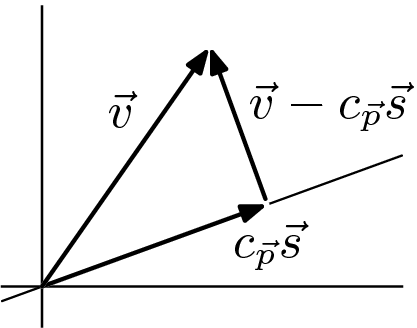
\includegraphics[width=0.5\textwidth]{Linalg_projection_4.png}
\end{figure}
\subsection{Linear least squares}
Let $\vect{A}$ be an $m\times n$ matrix, $\vect{x}$ be an $n\times 1$ matrix and b be an $m\times 1$ matrix. Solve the matrix equation $\vect{A}\vect{x}=\vect{b}$.\par 
If $m=n$, we can use three methods mentioned in section \ref{linear-eq}. However, if $m>n$, the the solution usually does not exist. But if the columns of $\vect{A}$ form a linearly independent set, then 
\begin{equation}
\dt{\trans{A}\vect{A}}\neq 0 \quad \text{and} \quad \trans{A}\vect{A}\vect{x}=\trans{A}\vect{b}
\end{equation}
\begin{equation}\label{least-square}
\vect{x}=\inverse{\trans{A}\vect{A}}\trans{A}\vect{b}
\end{equation}
The matrix equation now can be solved with the minimum error, meaning $\norm{\vect{A}\vect{x}-\vect{b}}$ is minimum. Using formula \eqref{least-square} to solve a system of equations is called The method of linear least squares.
\subsection{Rotation}
In linear algebra, a rotation matrix is a matrix that is used to perform a rotation in Euclidean space.
\subsubsection{In two dimensions}
In two dimensions, every rotation matrix has the following form,
\[ \vect{R}=\smtrx{\cos\alpha,-\sin\alpha\\ \sin\alpha,\cos\alpha} \]
rotates points in the xy-plane counterclockwise through an angle $\alpha$ about the origin of the Cartesian coordinate system. The column vectors are calculated by means of the following matrix multiplication,
\begin{equation*}
\cvect{x',y'}=\smtrx{\cos\alpha,-\sin\alpha\\ \sin\alpha,\cos\alpha}\cvect{x,y}
\end{equation*}
So the new coordinates $\left( x',y' \right)$ of the point $\left( x,y \right)$ after rotation are
are
\[
 x'=x\cos \alpha -y\sin \alpha \, \quad
 y'=x\sin \alpha +y\cos \alpha \,.
\]
\subsubsection{In three dimensions}
A basic rotation (also called elemental rotation) is a rotation about one of the axes of a Coordinate system. The following three basic rotation matrices rotate vectors by an angle $\theta$ about the x-, y-, or z-axis, in three dimensions, using the right-hand rule:
\[ {\begin{alignedat}{1}R_{x}(\theta )&={\begin{bmatrix}1&0&0\\0&\cos \theta &-\sin \theta \\[3pt]0&\sin \theta &\cos \theta \\[3pt]\end{bmatrix}}\\[6pt]R_{y}(\theta )&={\begin{bmatrix}\cos \theta &0&\sin \theta \\[3pt]0&1&0\\[3pt]-\sin \theta &0&\cos \theta \\\end{bmatrix}}\\[6pt]R_{z}(\theta )&={\begin{bmatrix}\cos \theta &-\sin \theta &0\\[3pt]\sin \theta &\cos \theta &0\\[3pt]0&0&1\\\end{bmatrix}}\end{alignedat}}\]
\section{Exercises}
\begin{exercise}
Consider an object living in 3D real place. Its current position is $P(2,5,3)$. The object is heading towards the point $Q(4,10,5)$, and moves to that direction exactly 3 length units. Calculate the position of this object after movement.
\end{exercise}

\begin{solution}
Let $\vect{y}$ be the vector of the movement and $\vect{x}$ be the distance between P and Q. We have:
\begin{meq*}
\vect{x} &=& \vect{Q}-\vect{P}=(4,10,5)-(2,5,3)=(2,5,2) \\
\norm{x} &=& \sqrt{2^2+5^2+2^2}=\sqrt{33},\quad \uvect{x}=\frac{1}{\sqrt{33}}(2,5,2) \\
\vect{y} &=& \vect{P}+3\uvect{x}=(2,5,3)+\frac{3}{\sqrt{33}}(2,5,2)
\end{meq*}
\end{solution}

\begin{exercise}
Let $\vect{a}=(2,4)$ and $\vect{b}=(1,-3)$ be vectors in $\mathbb{R}^2$. If these vectors are considered as edges of a parallelogram then calculate its area A. 
\end{exercise}

\begin{solution}
Let $\vect{A}$ be the matrix formed by $\vect{a}$ and $\vect{b}$
\[ \vect{A}=\smtrx{2,1\\4,-3} \]
The area of the parallelogram is the absolute value of the determinant of $\vect{A}$
\[ S=\vert \dt{A}\vert = \vert 2(-3)-4\cdot 1 \vert =10 \]
\end{solution}

\begin{exercise}
Suppose we want to draw a best fitting line through three points (4,-2), (5,0), (5,-1), (6,4), (7,5) and (8,5) so a linear function $y=t+kx$ should be given. Determine this function by means of the Method of Least Squares (LSM). Perform calculations by SAGE then plot points and the line in the same coordinate system.
\end{exercise}

\begin{solution}
The linear function $y=t+kx$ should satisfies the following system of equations with the minimum error:
\begin{equation}
\label{LSM-linear}
\begin{cases}
4k+t &= -2 \\
5k+t &= 0 \\
5k+t &= -1 \\
6k+t &= 4 \\
7k+t &= 5 \\
8k+t &= 5 
\end{cases}
\end{equation}
The equivalent matrix equation of \eqref{LSM-linear} is $\vect{A}\vect{x}=\vect{b}$, where
\[ \vect{A}=\smtrx{4,1\\5,1\\5,1\\6,1\\7,1\\8,1} \quad \vect{x}=\cvect{k,t} \quad \vect{b}=\cvect{-2,0,-1,4,5,5} \]
Using formula \eqref{least-square}, we now can perform calculations by SAGE as follow:
\begin{verbatim}
A=matrix([[4,1], [5,1], [5,1], [6,1], [7,1], [8,1]])
b=matrix([ [-2,0,-1,4,5,5] ]).T
x=(A.T*A).inverse() * (A.T*b)

k=x[0][0]
t=x[1][0]
z=var("z")

S=plot(k*z+t, (z,-1,9))
P = scatter_plot([[4,-2], [5,0], [5,-1], [6,4], [7,5], [8,5]])
show(S+P)
\end{verbatim}
\begin{tikzpicture}
\begin{axis}
[
    axis lines = middle,
    xlabel = {$x$}, ylabel = {$y$},
    xmin=-3,ymin=-3,xmax=10,ymax=6
]
%Below the red parabola is defined
\addplot [
    domain=3:10, 
    color=red,
]
{131/65*x-129/13};

%Here the blue parabloa is defined
\addplot[
    color=black,mark=square
    ]
coordinates {
(4,-2) (5,0) (5,-1) (6,4) (7,5) (8,5)
};
\end{axis}
\end{tikzpicture}
\end{solution}

\begin{exercise}
Suppose points (0,4),(1,8),(1,10),(2,5),(2,6), (8,10) and (6,10) are given. Approximate the points by a real trigonometric polynomial of degree 2. Plot the points and the
graph of this function in the same coordinate system. 
\end{exercise}

\begin{solution}
Suppose points (0,4),(1,8),(1,10),(2,5),(2,6), (8,10) and (6,10) are given. Approximate the points by a real trigonometric polynomial of degree 2. Plot the points and the
graph of this function in the same coordinate system. 
\end{solution}